\newcommand{\labtitle}{ECE/CS 5710/6710 - Modelsim Tutorial}
%\newcommand{\labdate}{}
\newcommand{\labsubtitle}{Modelsim Tutorial}
\vlsiheader


\section{Objective}
This documents shows the main steps for performing the simulation of VHDL or Verilog netlists. This step is crucial to ensure that your RTL code will behave correctly, before and after the synthesis and Place$\&$Route steps. The tool used Modelsim\textsuperscript{\tiny\textregistered} from Mentor Graphics. Keep in mind that this document simply gives a general overview and presents a basic case (a verilog 2-input xor module) so you can get an idea of how to use the tool for your project. There are many other possibilities when using the tools that you will probably learn by yourself when working with it.

\section{Simulating the RTL Code}
\section{Starting the Tool}

 To launch modelsim, go to your \textit{modelsim} directory and do:
\begin{codeline}
	vsim
\end{codeline}


\section{Creating a New Project}
Modelsim\textsuperscript{\tiny\textregistered} allows you to work with project to organize your files. It is generally a good practice to have a project dedicated for each design. For instance, in this lab, you will create a specific project but you should create a new one for your class project later on. To create a new project:
\begin{enumerate}
	\parbox[t]{\dimexpr\textwidth-\leftmargin}{%		
	\begin{wrapfigure}[20]{r}{0.45\textwidth}
		\vspace{0mm}
		\centering
		\vspace{-\baselineskip}
		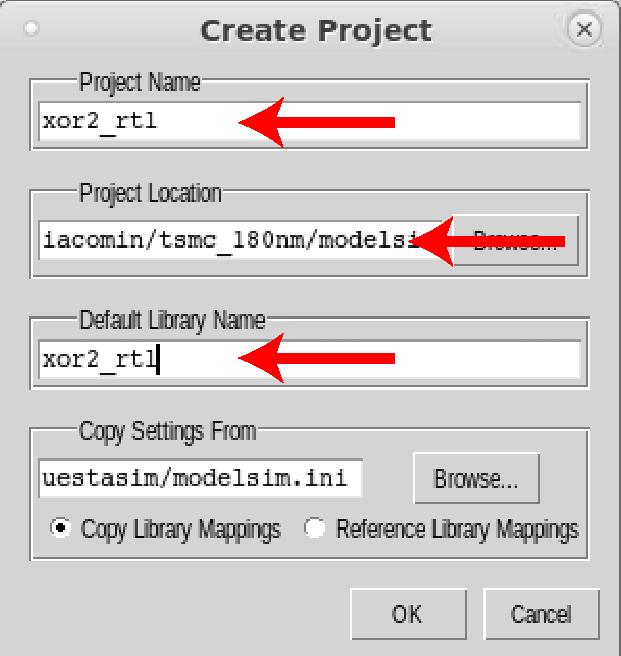
\includegraphics[scale=0.5]{figures/modelsim/create_project.pdf}
		\caption{Creating a new project.}
		\label{create}
	\end{wrapfigure}
	\item Go to \textit{File -> New -> Project}.
\item Define the following settings:
\begin{itemize}
	\item \textit{Project Name}:  xor2$\_$rtl
	\item \textit{Project Location}: ...../PROJECTS
	\item \textit{Default Library Name}: xor2$\_$rtl (it is a good idea to use the same name as your projectname).
	%\item \textit{Copy Settings From:}: .../modelsim.ini
	\item Select Copy Library Mappings
\end{itemize}
\item Click OK.
}
\end{enumerate}
		\vspace{10mm}




\section{Adding the RTL Files}
A window should pop up. From there, you can either create a new file for your RTL code or import existing ones. For this tutorial, you will import two files: a verilog file describing the RTL code of a 2-input xor function and a verilog file for its testbench. To do so:hots of the appropriate reports).

\begin{enumerate}
	\parbox[t]{\dimexpr\textwidth-\leftmargin}{%		
	\begin{wrapfigure}[20]{r}{0.45\textwidth}
		\vspace{0mm}
		\centering
		\vspace{-\baselineskip}
		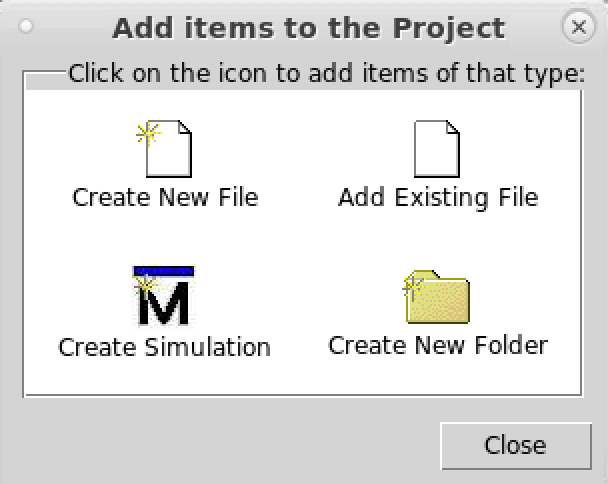
\includegraphics[scale=0.5]{figures/modelsim/add_file}
		\caption{Creating a new project.}
		\label{addfile}
	\end{wrapfigure}
	\item Click on \textit{Add Existing File}.
\item A new window opens. Click on browse and go to your \textit{HDL/RTL} folder. Select both \textit{xor2.v} and \textit{xor2$\_$tb.v} files.
\item Click on \textit{Open} and then \textit{Ok}.
\item You can then close the \textit{Add items to the Project} Window.
\item You should be able to see the 2 verilog files in the main window.
}
\end{enumerate}



\section{Compiling the Files}
Now, you need to compile the files. This step will check for errors in your verilog code and let you know if there are any.

\begin{remark}
When working on your class project, it is suggested to change the project settings to allow compilation messages to appear in the \textbf{\textcolor{blue}{Transcript pane.}} To do so, go to: \textit{Project -> Project Settings...}, check the \textit{Display compiler output} box and click \textit{Ok}.
\end{remark}

	\parbox[t]{\dimexpr\textwidth-\leftmargin}{%		
	\begin{wrapfigure}[20]{r}{0.55\textwidth}
		\vspace{0mm}
		\centering
		\vspace{-\baselineskip}
	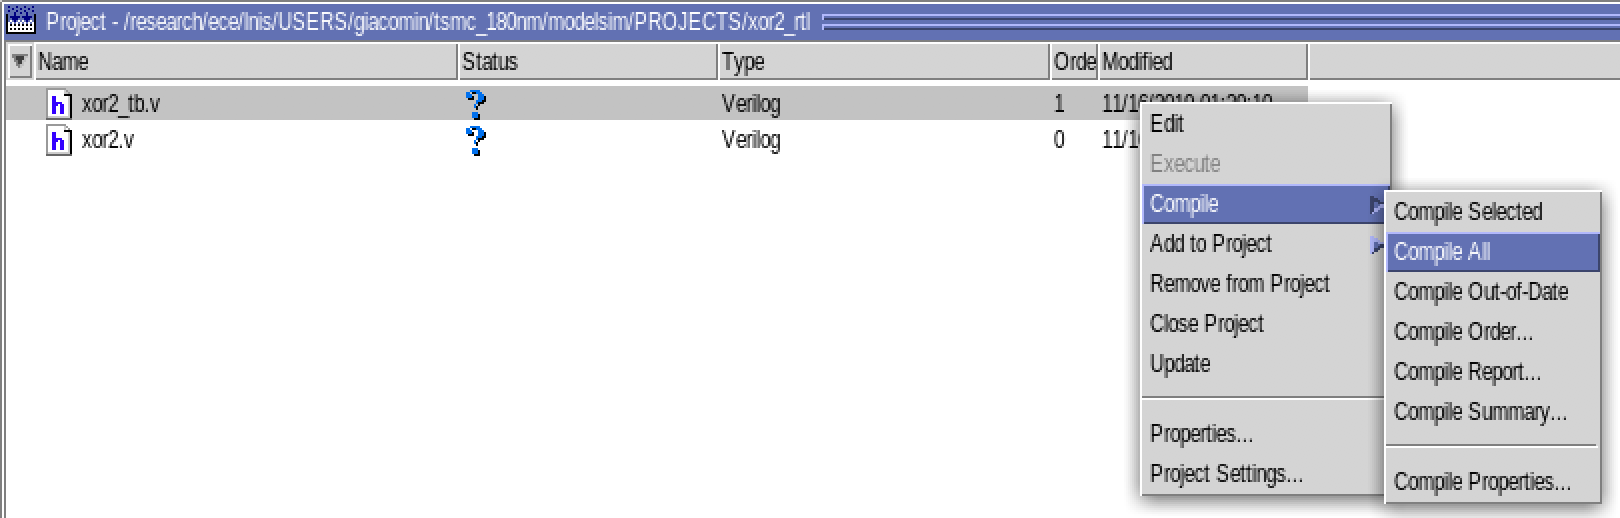
\includegraphics[scale=0.35]{figures/modelsim/compile}
	\caption{Compiling the files.}
\label{compile}
	\end{wrapfigure}
In the \textit{Project} tab, right click and select: \textit{Compile -> Compile All}. \newline
If there is no compilation error, each file status becomes OK (\img{figures/modelsim/good}). If there are some errors, the status is \img{figures/modelsim/bad}. Compilation error messages are displayed in red in the console pane. If you double click on those, it will open the editor pane and highlights the line causing the error.
}
\clearpage
\section{Defining the Simulation Configuration}
This step will define all the necessary settings required to perform the RTL simulation. To do so:


\begin{enumerate}
	\parbox[t]{\dimexpr\textwidth-\leftmargin}{%		
		\begin{wrapfigure}[20]{r}{0.55\textwidth}
			\vspace{0mm}
			\centering
			\vspace{-\baselineskip}
			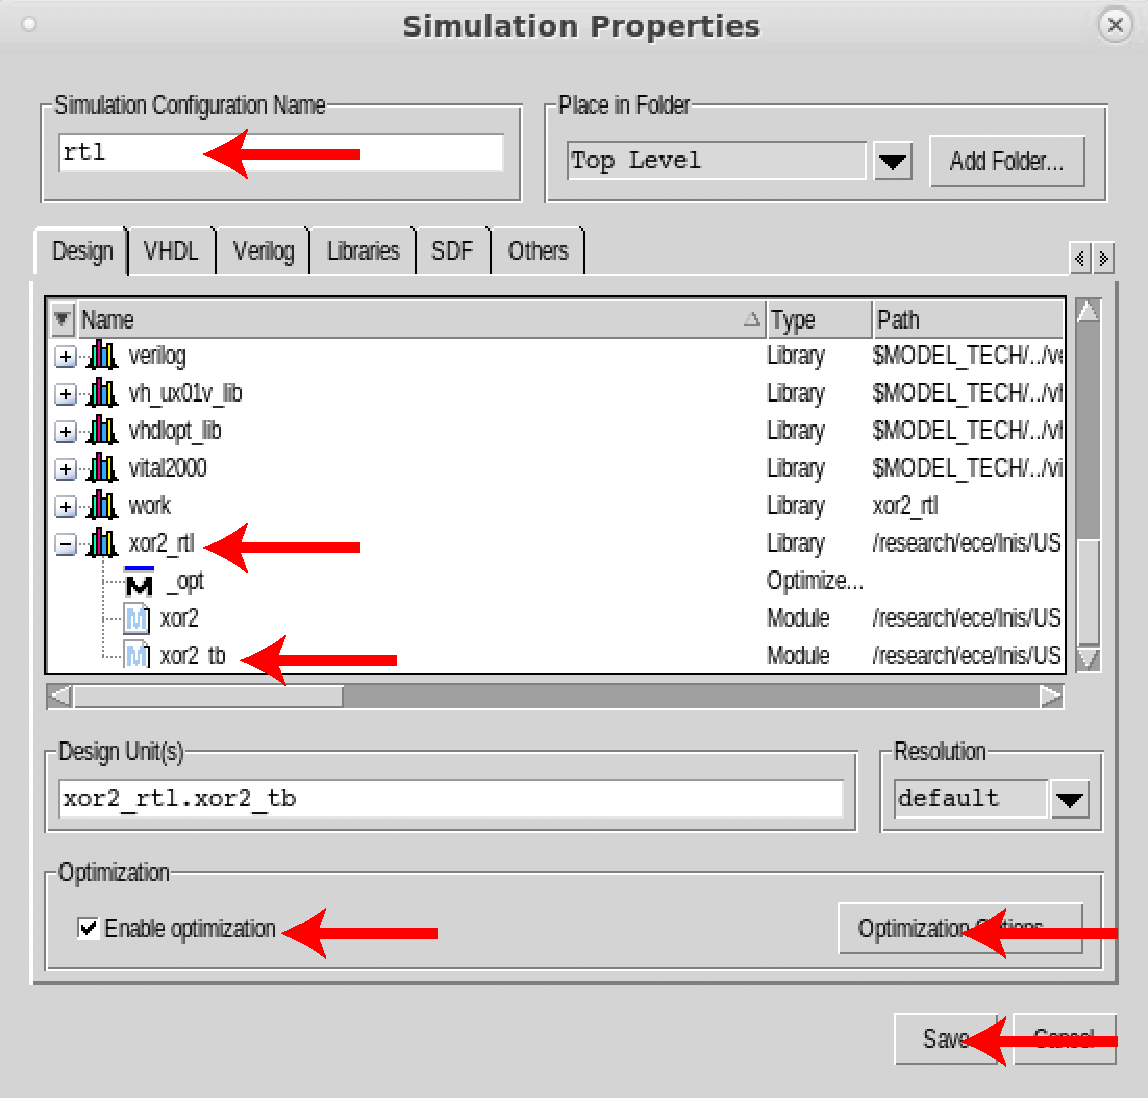
\includegraphics[scale=0.44]{figures/modelsim/create_settings.pdf}
			\caption{Creating a simulation configuration.}
			\label{compile}
		\end{wrapfigure}
	\item Go to: \textit{Project -> Add to Project -> Simulation Configuration....}
	\item Define the following settings:\footnote{This is your testbench module.}
	\begin{itemize}
		\item \textit{Simulation Configuration Name}:  rtl
		\item \textit{Resolution}: ns
		\item \textit{In the Design Tab}: Select the configuration declaration \textit{xor2$\_$tb} (this is your testbench module) in the \textit{xor2$\_$rtl} (that you defined when creating your project) design library.
		\item \textit{Optimization Options... }: Click here and select \textit{Apply full visibility to all modules} so all the signals will be available to be displayed when doing the simulation.
		\item Click on \textit{Save}.
	\end{itemize}
	}
\item You should be able to see the simulation icon (\img{figures/modelsim/simconf}) in the \textit{Project} tab.
\end{enumerate}


\section{Running the Simulation}

To start the simulation, double click on the simulation configuration icon (\img{figures/modelsim/simconf}) in the \textit{Project} tab. A new \textit{sim} tab should appear in the Modelsim\textsuperscript{\tiny\textregistered} window, as shown in Fig. \ref{sim_modelsim_window}. This tab includes all the simulation hierarchy (such as the different modules, the statements, \textit{etc.}). 

\begin{figure}[!h]
	\centering
	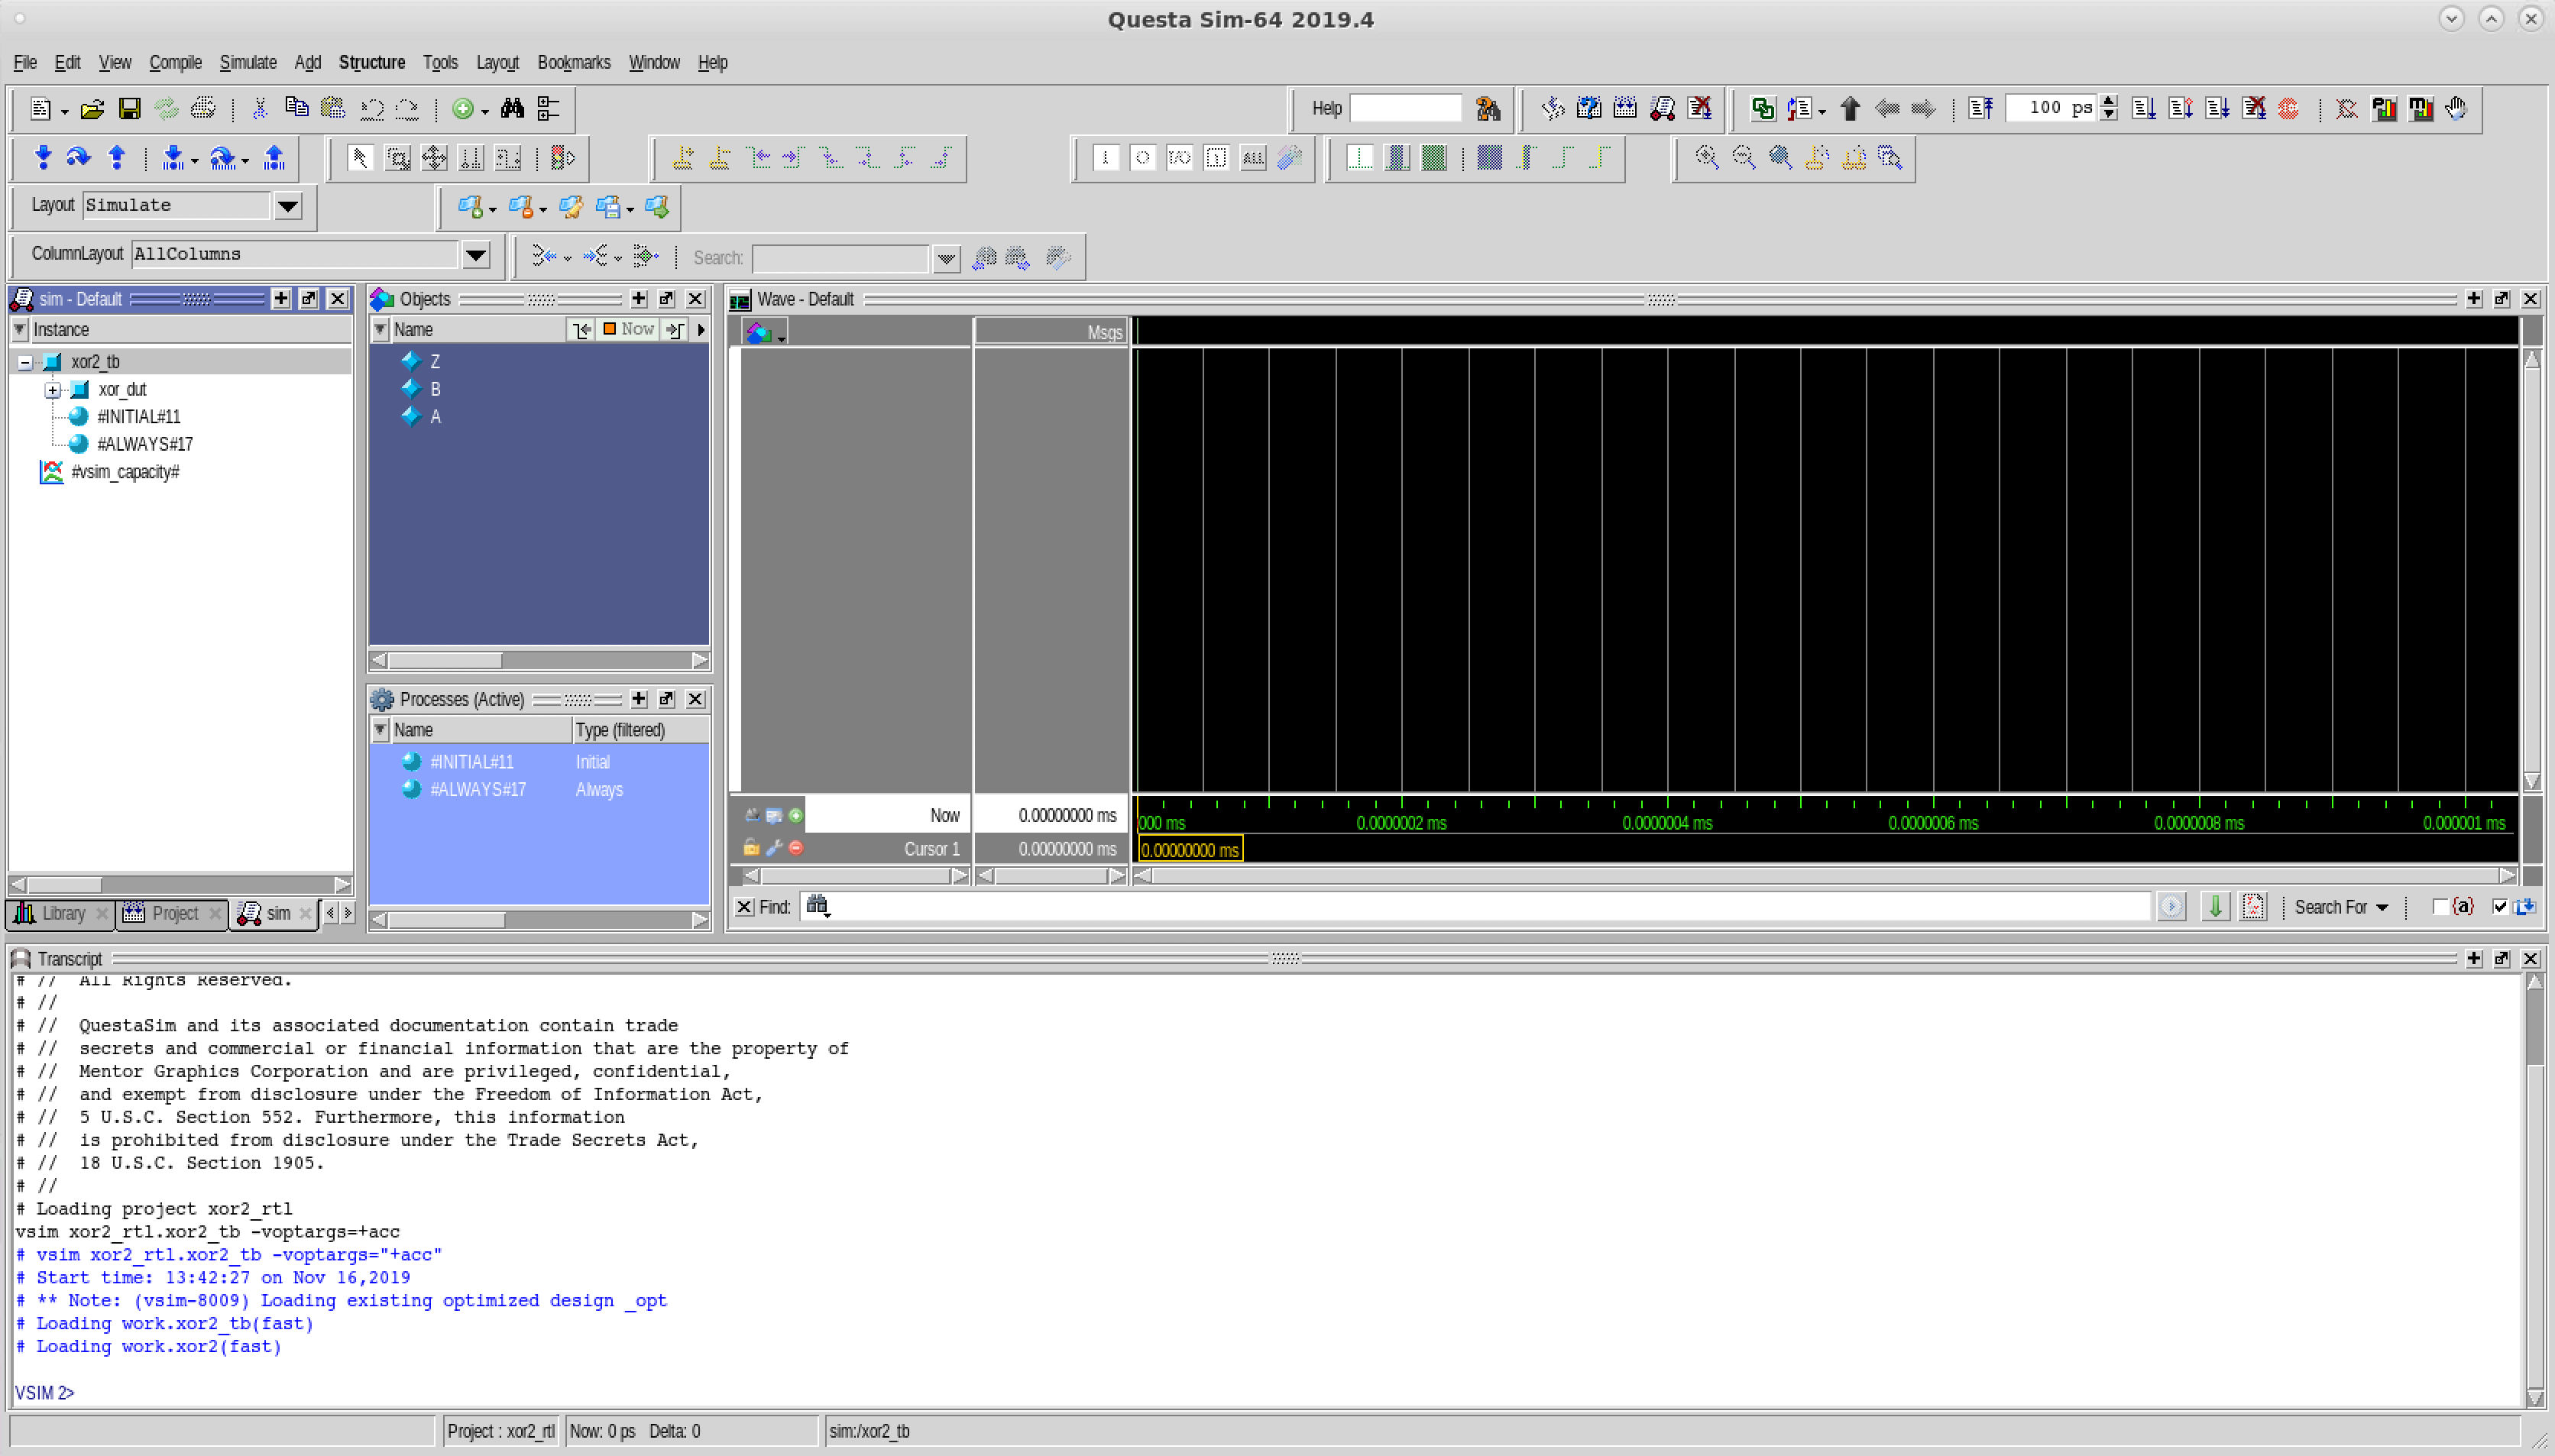
\includegraphics[scale=0.28]{figures/modelsim/post_sim}
	\caption{Modelsim\textsuperscript{\tiny\textregistered} window after doing the simulation. }
	\label{sim_modelsim_window}
\end{figure}

Now, select the signals to be displayed. In the \textit{Objects} pane, select the signals you want to display, right click and do: \textit{Add Wave}. You can also display all the top level signals of your testbench by going to the \textit{sim} pane, right clicking on the top level module (\textit{xor2$\_$tb} in this case) and do: \textit{Add Wave}. You should now be able to see the signal list in the \textit{wave} pane. \\
To launch the simulation:

\begin{enumerate}
	\parbox[t]{\dimexpr\textwidth-\leftmargin}{%		
		\begin{wrapfigure}[20]{r}{0.4\textwidth}
			\vspace{0mm}
			\centering
			\vspace{-\baselineskip}
			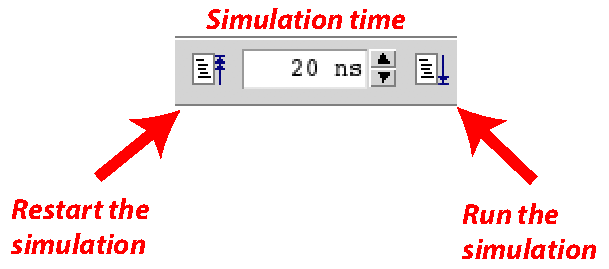
\includegraphics[scale=0.5]{figures/modelsim/runsim.pdf}
			\caption{Simulation toolbox.}
			\label{compile}
		\end{wrapfigure}
		\item Specify a simulation time (which should makes sense for the defined testbench).
		\item Click on \textit{Run}.
		\item In case you modify your verilog file, you can select \textit{Restart} to clean the simulation output pane and restart the simulation.
	}

\end{enumerate}
	You can also run the simulation by using the \textbf{\textcolor{blue}{Transcript pane.}}:
\begin{codeline}
	run 10ns
\end{codeline}
	To restart the simulation, you can also use:
\begin{codeline}
	restart -f
\end{codeline}

Now, you should be able to see the displayed results. In some cases, you might need to change the radix of a variable (to decimal, hexadecimal, signed , \textit{etc.}). To do so: In the \textit{Wave} window, click on the signal or the variable and select \textit{Radix -> radix name}.

\begin{figure}[!h]
	\centering
	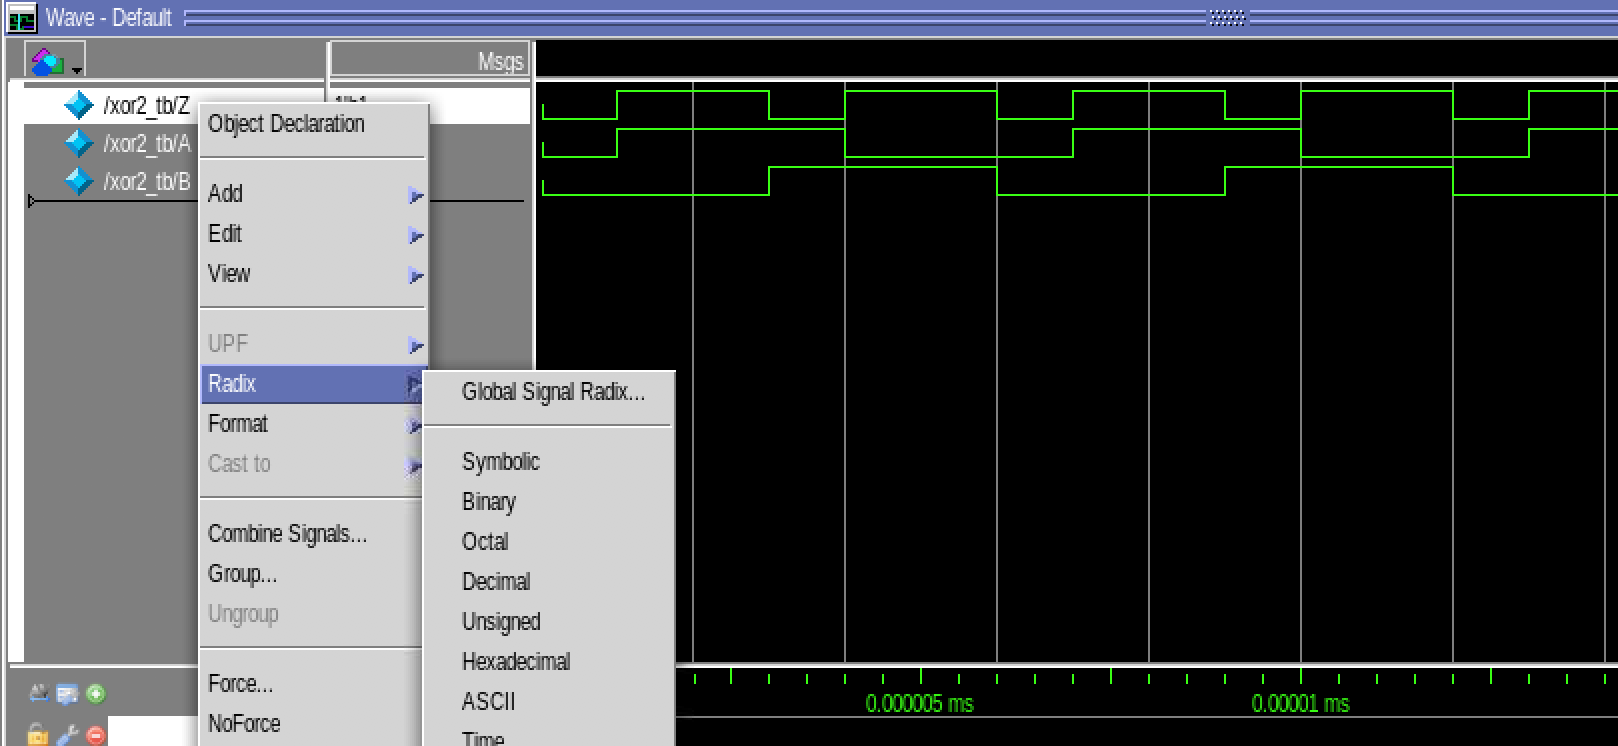
\includegraphics[scale=0.4]{figures/modelsim/radix}
	\caption{Change the radix of a variable.}
	\label{outputwave}
\end{figure}

\section{Modifying the RTL files}
For this tutorial, the two provided files show the behavior of a XOR so you do not have to modify those. However, for your project, you probably will have to write some verilog code yourself and modify it many times, after realizing that the simulation does not behave as intended. To flow is generally the following:

\begin{enumerate}
	\item You can modify any verilog files which are in your current project by double clicking on it. A new window will open where you can make your changes. Once you are done, save the file.
	\item You then need to re-compile the changed files, as explained previously.
	\item Then you need to launch the simulation. If a simulation was already opened, you do not need to double click on the the simulation icon (\img{figures/modelsim/simconf}) in the \textit{Project} tab to relaunch it. You simply need to restart (\img{figures/modelsim/restart}) your simulation, and re-run (\img{figures/modelsim/rerun}) it again.
	\item Verify if the simulation behaves as expected and reiterate the previous steps if necessary.
	\item For your testbenches, thos one have to be carefully written. As you did in Virtuoso\textsuperscript{\tiny\textregistered} for your electrical simulations, you have to make sure that you test all (or as much as possible) the possible input cases to ensure that your system behaves correctly. For instance, in this tutorial, you should check on the XOR output curves that the 4 input cases (00, 01, 10, 11) are all simulated and shows a correct XOR output.
\end{enumerate}

\section{Post-Synthesis and P$\&$R Functional Verification}
After the design has been synthesized, you should perform another simulation to ensure that it still behave correctly. Below are some general guidelines:
	\begin{enumerate}
		\item You will need to create a new project. The RTL and post-synthesis simulations each need to be separate. As such, you can for instance replace \textit{xor2$\_$rtl} by \textit{xor2$\_$mapped} for the project name, library name, etc.
		\item The verilog files to include are different: you will need to include the mapped netlist you obtained after running Design Compiler (in the HDL/GATE folder). You also need to include the Verilog standard cell library which describe the behavior of the standard cells you used to synthesize your design. The file path is: \\
		\textit{/research/ece/lnis-teaching/Designkits/tsmc180nm/full$\_$custom$\_$lib/verilog/sclib$\_$tsmc180.v}. \\ Finally, you need to include your testbench, which should be the same as for your RTL simulation.
		\item When creating the simulation configuration, you also need to link the SDF file. This file will back annotate your mapped Verilog netlist in order to represent the delays from the logic gates of your designs. To do so:
			\begin{enumerate}
				\item As before, create a new simulation configuration and choose its name. Select the design unit as shown in the picture from the appropriate library. Don't forget to apply the full visibility to all modules as before.
				\item Go to the SDF tab, and click on \textit{Add..}
				\item Browse to select the SDF file created by the synthesis step (located in the \textit{design$\_$compiler/SDF folder}).
				\item The \textit{Apply to Region} field should be \textit{xor2$\_$tb/xor2$\_$dut} where \textit{xor2$\_$tb} is the name of your top verilog testbench module \textit{xor2$\_$dut} is the name of the instantiated module in your testbench.
				\item Click on \textit{OK} and \textit{Save}.
				\end{enumerate}
		\begin{figure}[!h]
			\centering
			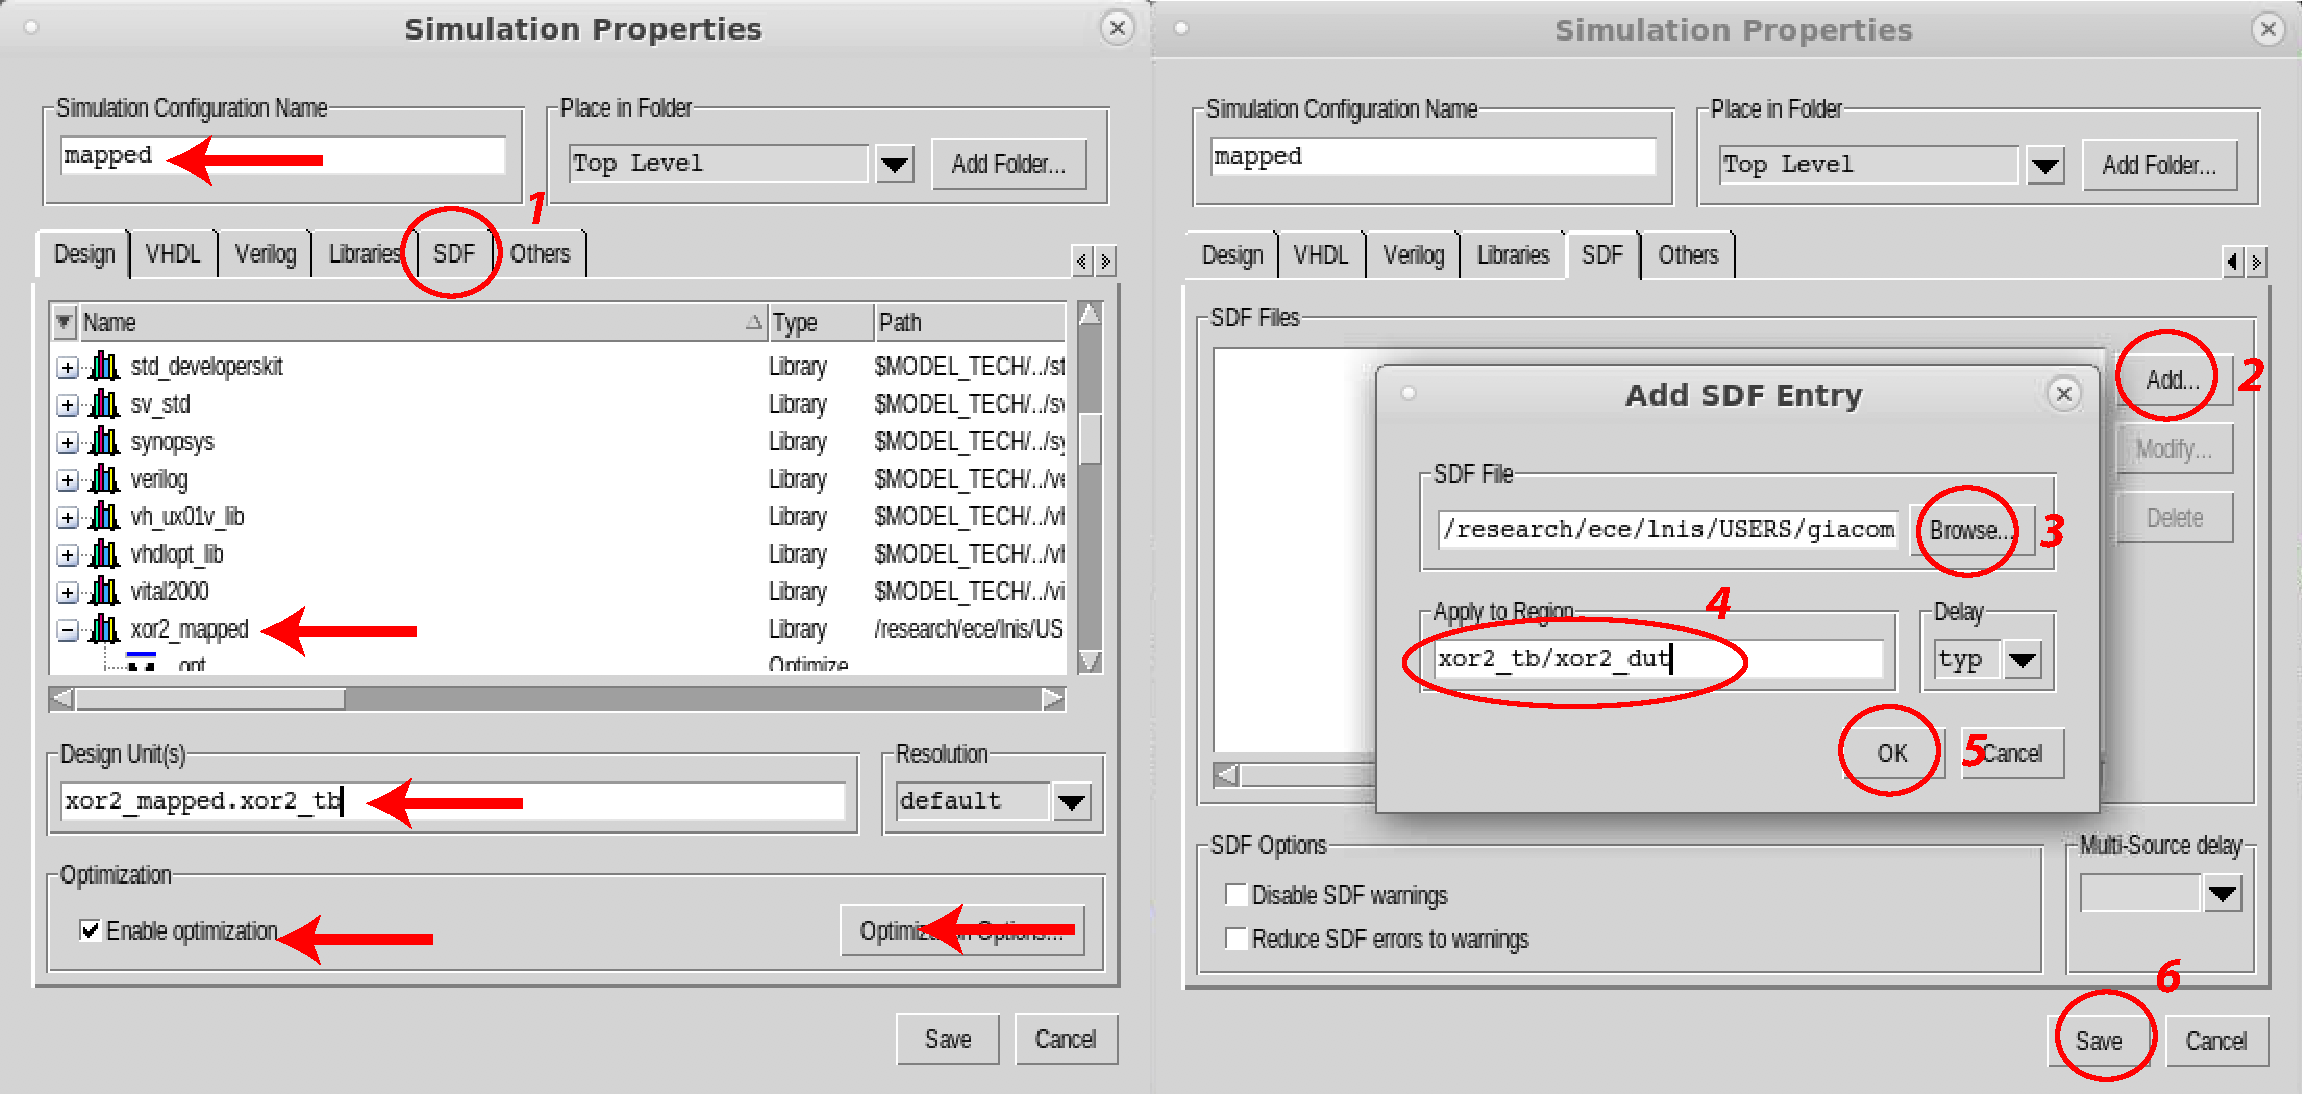
\includegraphics[scale=0.4]{figures/modelsim/sdf_settings.pdf}
			\caption{Post-synthesis simulation configuration.}
			\label{sdf}
		\end{figure}
	\item For the post-P$\&$R simulation, you will need to repeat this step. Don't forget to create another project. When adding the verilog files to your project, also add the pad library verilog file: \\
			\textit{/research/ece/lnis-teaching/Designkits/tsmc180nm/full$\_$custom$\_$lib/verilog/padlib$\_$tsmc180.v}. 
		\end{enumerate}
	
	\begin{remark}
		When doing post-synthesis and P$\&$R simulations, don't forget to specify in your testbench the same period that you specified to constrain your design when synthesizing.
	\end{remark}